\documentclass[a4paper,12pt,onecolumn,twoside,openright]{book}



\usepackage[english, italian]{babel}

\usepackage[utf8]{inputenc}
\usepackage[T1]{fontenc}
\usepackage{graphicx}
\usepackage{verbatim}
\usepackage[bookmarks=true, hidelinks]{hyperref}

\usepackage{color}
\usepackage[italian]{nomencl}
\usepackage{caption}
\usepackage{booktabs}
\usepackage{tabularx}
\usepackage{tabulary}
\usepackage{multirow}
\usepackage{longtable}
\usepackage{tabu}
\usepackage{float}
\usepackage{subfig}
\usepackage{listings}

%-----python------------------

\definecolor{deepblue}{rgb}{0,0,0.5}
\definecolor{deepred}{rgb}{0.6,0,0}
\definecolor{deepgreen}{rgb}{0,0.5,0}
\definecolor{gray}{rgb}{0.5,0.5,0.5}
\definecolor{lightgray}{rgb}{0.95,0.95,0.8}

% Python style for highlighting

\lstset{frame=tb,
	language=Python,
	aboveskip=3mm,
	belowskip=3mm,
	showstringspaces=false,
	columns=flexible,
	basicstyle={\small\ttfamily},
	numbers=none,
	numberstyle=\tiny\color{gray},
	keywordstyle=\color{deepblue},
	commentstyle=\color{deepred},
	stringstyle=\color{deepgreen},
	breaklines=true,
	breakatwhitespace=true,
	tabsize=3,
	backgroundcolor = \color{lightgray}
}
%--------Lettere greche non in italic----------------------------
\usepackage{upgreek}

%--------Faccio andare a capo gli url anche con - e / -----------
\usepackage{url}

%----------------------------------------------------------------

\setlength{\topmargin}{0.0cm} \setlength{\evensidemargin}{+0.95cm}
\setlength{\oddsidemargin}{+0.95 true cm}

\usepackage{etoolbox}% http://ctan.org/pkg/etoolbox
\makeatletter

\patchcmd{\@makechapterhead}{50\p@}{\chapheadtopskip}{}{}% Space from top of page to CHAPTER X
\patchcmd{\@makeschapterhead}{50\p@}{\chapheadtopskip}{}{}% Space from top of page to CHAPTER X

\makeatother
\newlength{\chapheadtopskip}\setlength{\chapheadtopskip}{20pt}

%----------------------------------------------------------------

%------Imposto larghezza ed altezza del testo--------------------
\setlength{\textwidth}{14cm} \setlength{\textheight}{22cm}
\setlength{\headheight}{26pt}
%----------------------------------------------------------------

%------Setto interlineare ad 1 riga e 1/2------------------------
\linespread{1.3}

%----------------------------------------------------------------

%------------------------------------------------------------------


%\makenomenclature

\begin{document}
	
	\selectlanguage{Italian}
	
	\hypersetup{pageanchor=false}
	\begin{titlepage}
$\;$
 \vspace{-1.0 true cm}
\begin{center}
    {\large  \textsc{Alma Mater Studiorum - Universit\`{a} di Bologna}} \\
    \rule{13.2cm}{.5pt} \\
    \vspace{3mm}
  {\normalsize \textsc {Scuola di Ingegneria \\
  	Dipartimento dell'Energia elettrica e dell'Informazione \\
    "Guglielmo Marconi" DEI} \\
  \vspace{1.0 true cm}
  Corso di Laurea in \\
  Ingegneria Elettronica e Telecomunicazioni \\
  \vspace{5mm}
  Tesi di Laurea in \\
  Calcolatori Elettronici}
\end{center}

\vspace{2.5 true cm}

\begin{center}
    {\Large \textbf{Strumento per annotazione semantica 3D
    \\ \vspace{0.3cm}con realtà virtuale}}

    \vspace{2.5 cm}
\end{center}


\vfill \normalsize {
    \begin{tabular}{lr}
        Candidato:      &  \hspace{5cm} Relatore:    \\
    \textbf{Luigi Lella}         &  Ch.mo prof. \textbf{Luigi Di Stefano} \\	
          &  \hspace{8cm} Correlatore:    \\
    \label{key}      &  \hspace{5cm} \textbf{Pierluigi Zama Ramirez}    \\
    						       
    \end{tabular}
} \vspace{2.5 cm}



%\renewcommand{\baselinestretch}{2.0}
 \rule{13.2cm}{.5pt}
 \small
 \begin{center}
 \normalsize Anno Accademico 2019/2020 \\
 \end{center}
\begin{center}
	\normalsize Sessione IV \\
\end{center}


\end{titlepage}


	
	%------ Parole Chiave ------------------------------------------------
	
	\newpage
	\thispagestyle{empty} $\;$
	\newpage
	
	\setcounter{tocdepth}{3}
	%----------------------------------------------------------------------------------
	
	\hypersetup{pageanchor=true}
	
	\pagenumbering{roman}
	
	
	%------------------------Creo l'indice---------------------------------------------
	
	\tableofcontents \cleardoublepage
	
	\listoffigures \cleardoublepage
	
%	\listoftables \cleardoublepage
	
	%-------- Setto il contatore delle pagine ad 1----------------------
	\setcounter{page}{1}
	%------------------------------------------------------------------
	
	%------ Imposto il contatore delle pagine --------------------------
	%       in formato arabico
	\pagenumbering{arabic}
	
	%-----  Includo i capitoli e appendici -----------------------------
	
	\chapter*{Introduzione}
\addcontentsline{toc}{chapter}{Introduzione}
\phantomsection
\chaptermark{Introduzione}

Negli ultimi anni machine learning e deep learning hanno rivoluzionato il mondo dell'intelligenza artificiale e della computer vision ottenendo risultati impressionanti in molti compiti come classificazione di immagini, segmentazione semantica ecc. superando, in alcuni casi, anche i risultati ottenuti da un utente umano in precisione e accuratezza \cite{imagenet}.\\
Per usare tutti questi strumenti abbiamo bisogno di una grande quantità di dati al fine di supervisionare la parte di training. Per questa ragione sono stati creati innumerevoli dataset contenenti dati grezzi e le rispettive annotazioni come ad esempio KITTI \cite{KITTI}, Matterport3D \cite{Matter} e Replica \cite{Replica}.\\\
La fase di annotazione, come si può facilmente immaginare, è però un processo lento, noioso e molto propenso ad errori. Labellare una singola immagine in 2D può richiedere alcune ore ed è un compito che richiede anche una certa esperienza con l'utilizzo di alcuni software. La difficoltà poi cresce se decido di lavorare con dati 3D come mesh o pointcloud.\\\\
Per semplificare e velocizzare questa parte si è deciso di realizzare \textit{Shooting Labels} un tool per la segmentazione semantica 3D basato su realtà virtuale. L'utente viene trasportato all'interno di una scena rappresentata come mesh 3D, dove tutte le superfici possono essere "colorate" semanticamente. L'esperienza immersiva fornita dalle tecnologie VR consente all' utente di muoversi fisicamente all'interno dello scenario etichettare e interagire con gli oggetti in modo naturale e coinvolgente rendendo questo compito, oltre che più veloce, anche divertente come giocare a un video-game \cite{SL}.\\\\
In questo elaborato si parlerà dapprima della segmentazione semantica e dei problemi di ottenere dati con cui allenare una rete, verranno poi presentati gli strumenti utilizzati nel corso della stesura della tesi e tirocinio per poi passare ad una trattazione dettagliata del software. Infine verranno analizzati e commentati alcuni dati ottenuti dall'utilizzo di questo strumento.
	\chapter{Il Network Slicing}\label{ch:capitolo1}

\section{Concetti principali}\label{ch:1.1}
La sempre più rapida evoluzione e innovazione delle tecnologie ha portato, negli anni, a modificare radicalmente le prestazioni ed i servizi richiesti alle infrastrutture di telecomunicazioni.\\
Internet, che ad oggi risulta la rete più diffusa al mondo, non rispecchia più le necessità  degli utilizzatori. Alla sua nascita, infatti, la Qualità del Servizio (QoS) richiesta era decisamente inferiore. Per questo motivo, la filosofia su cui è basato Internet è detta \textit{best-effort}: il sistema farà tutto il possibile per compiere un'operazione, ma non è garantito se e come questa sarà portata a termine.\\
Tuttavia, l'evoluzione di applicazioni e servizi ha reso necessaria una maggiore flessibilità delle prestazioni fornite dalla rete. A seconda dei casi, infatti, un servizio potrebbe richiedere bassa latenza, altri potrebbero avere bisogno di alto throughput. L'architettura e i protocolli di Internet non sono pensati per questo scopo e fornire prestazioni di questo tipo richiederebbe modifiche sostanziali.
\cite{libro1}\\
Da queste necessità nasce l'idea del Network Slicing.\\
Una \textit{Network slice} è un insieme di risorse che compongono una rete in grado di soddisfare le necessità di una specifica applicazione. Questo comportamento si può ottenere utilizzando diverse architetture e tecnologie che, insieme, ci permettono di manipolare il comportamento della rete.\\

\subsection{Software Defined Networking}\label{ch:1.1.1} 
Uno dei concetti alla base dell'idea del NS è il \textit{Software Defined Networking (SDN)}, ovvero la costruzione di reti in cui il \textit{routing} ed il \textit{forwarding} sono gestiti separatamente.\\
L'SDN prevede infatti la presenza di uno o più controller, che gestiscono il routing ed il comportamento complessivo della rete. I vantaggi che un approccio di questo tipo comporta sono molteplici.
\begin{itemize}
	
	\item La rete non è vincolata all'infrastruttura fisica. Il suo comportamento, definito via software, può quindi essere facilmente modificato e riprogrammato.
	
	\item La centralizzazione dell'intelligenza della rete stessa permette al gestore di operare solo sul controller, senza la necessità di intervenire su ogni singolo nodo. Inoltre, il controller permette di monitorare e supervisionare agevolmente l'intera infrastruttura \cite{6461195}	
	
\end{itemize}
\begin{figure}[h!]
	\centering
	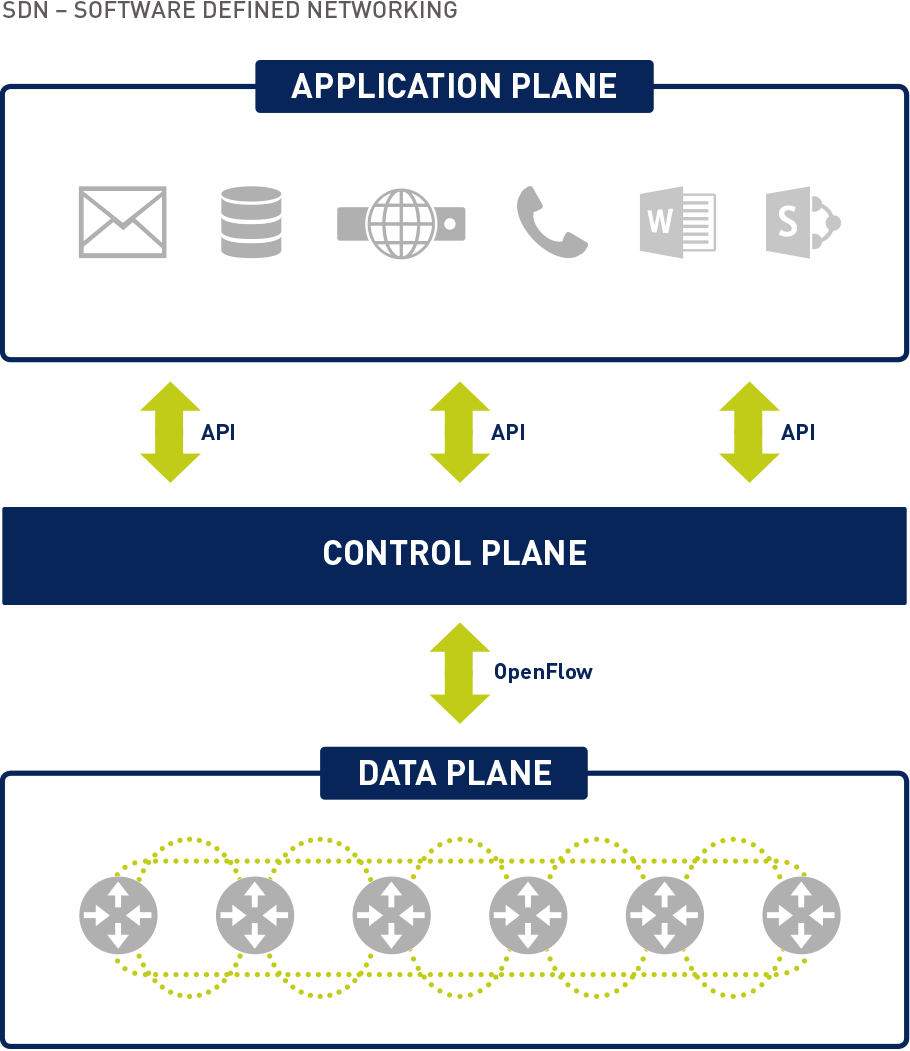
\includegraphics[width=0.6\linewidth]{../immagini/552578-sdn-graphic-blue-910}
	\caption[Software Defined Network]{Gestione software dell'infrastruttura fisica in una rete di tipo SDN}
	\label{fig:552578-sdn-graphic-blue-910}
\end{figure}

\subsection{Virtualized Network Functions}\label{ch:1.1.2}
Un altro elemento cardine per il Network Slicing è la \textit{virtualizzazione delle funzioni di rete (NFV)}. Le funzioni di rete, infatti, vengono solitamente implementate tramite hardware specifico in ogni nodo. Gli svantaggi di questa architettura includono l'alto prezzo dell'energia necessaria, un maggiore costo dovuto alla progettazione ed alla produzione dell'hardware stesso e l'inevitabile sempre più corto ciclo di vita di quest'ultimo.\\
La NFV si pone come obiettivo la soluzione di questi problemi, implementando le stesse funzioni di rete tramite software. Le \textit{funzioni di rete virtualizzate} non necessitano quindi di una specifica infrastruttura fisica, ma sono in grado di essere memorizzate ed eseguite da generici switch, server e data center, tramite la creazione su di essi di una o più macchine virtuali. Questo, insieme alla possibilità di poter spostare questi elementi hardware in qualunque nodo della rete, rende estremamente più pratica, economica ed efficiente la gestione della rete stessa. \cite{telecom_nfv}
\begin{figure}[h!]
	\centering
	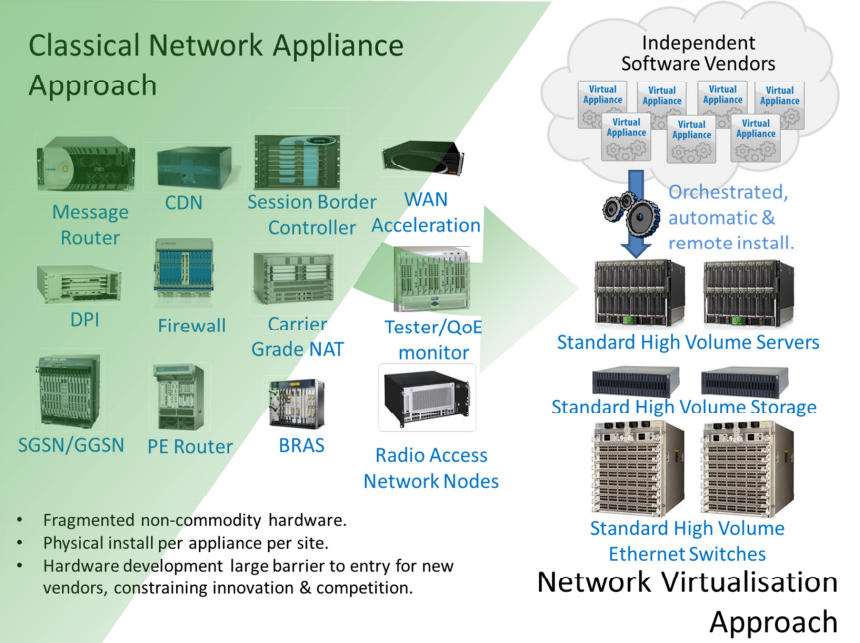
\includegraphics[width=0.8\linewidth]{../immagini/nfv}
	\caption[Network Function Virtualization, NFV]{Differenze tra l'hardware specifico richiesto normalmente dalle funzioni di rete e da quello generico utilizzato dalle VNF}
	\label{fig:nfv}
\end{figure}

\section{Architetture}\label{ch:1.2}
Lo scopo del Network Slicing è fare in modo che un'infrastruttura possa suddividere e organizzare le proprie risorse affinché un'applicazione abbia a disposizione una rete ottimizzata per le sue richieste.\\
Per fare ciò, queste architetture sono strutturate su 3 livelli:
\begin{itemize}
	
	\item \textit{Service Instance Layer}\\
	Rappresenta il servizio che deve essere supportato dalla rete. Ogni servizio è rappresentato da una Service Instance.
	
	\item \textit{Network Slice Instance Layer}\\
	Racchiude i vari Network Slices, ovvero le risorse allocate per una determinata Service Instance. Una Network Slice Instance può essere condivisa tra più SI.
	
	\item \textit{Resource Layer}\\
	Rappresenta le risorse e le funzioni di rete disponibili sull'infrastruttura, che verranno suddivise e assegnate in base al servizio richiesto.
	
	
\end{itemize}
L'intera architettura viene "orchestrata" da uno o più \textit{controller}, che hanno il compito di creare e organizzare le varie Istanze, stanziando le risorse necessarie per ciascun servizio.
\cite{NSintro}
\begin{figure}
	\centering
	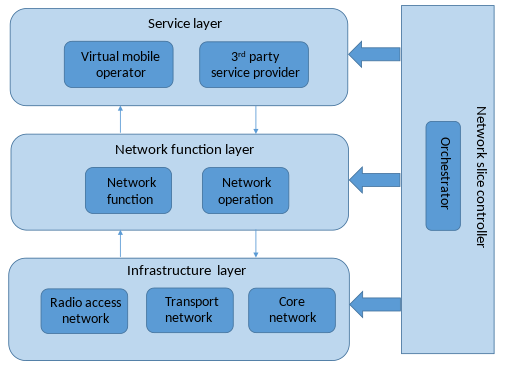
\includegraphics[width=0.9\linewidth]{../immagini/510px-Generic_5G_network_slicing_framework.svg}
	\caption[Architettura Network Slicing]{Struttura delle architetture di rete basate sul Network Slicing}
	\label{fig:510px-generic5gnetworkslicingframework}
\end{figure}\\
L'utilizzo di un solo controller può costituire un collo di bottiglia per le prestazioni della rete in caso di compiti particolarmente complessi. Per questo motivo può risultare efficace dividere i compiti tra più controller, assegnando a ciascuno la gestione di determinate funzionalità.
\begin{figure}
	\centering
	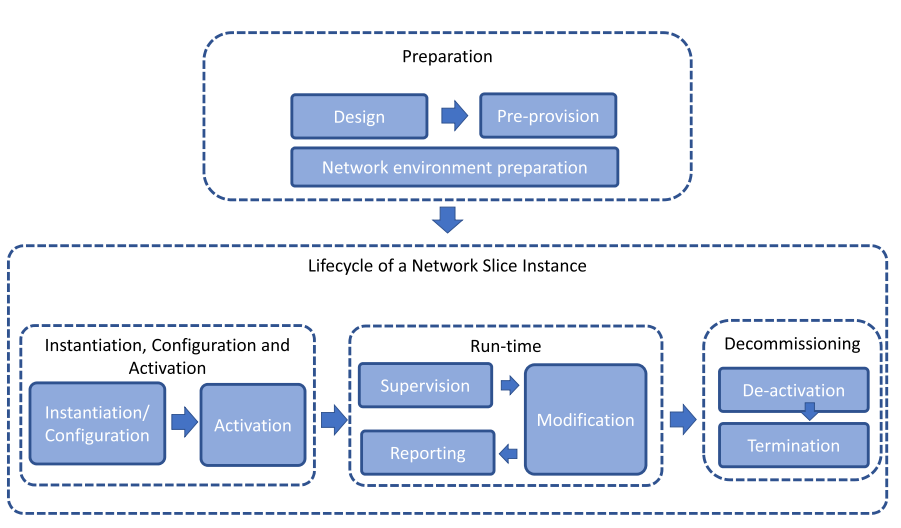
\includegraphics[width=1\linewidth]{../immagini/nslc}
	\caption[Network Slice life cycle]{Life Cycle di una Network Slice Instance}
	\label{fig:nslc}
\end{figure}\\\\
Il processo di creazione di un'Istanza inizia con un'operazione di progettazione e preparazione della stessa. Viene poi effettuata una richiesta di creazione, e attivazione della Slice. Una volta attivata, questa viene monitorata e modificata. Quando non è più necessaria, infine, viene disattivata e le risorse vengono rese nuovamente disponibili.\\\\
È importante sottolineare come le Slices siano tra loro isolate. Questo è un criterio fondamentale, che permette una maggiore privacy, impedendo di accedere ai dati delle altre Slices, e garantisce che le prestazioni di una Slice non influiscano sulle altre.\\\\
Il Network Slicing può essere implementato  in diversi modi. Un'infrastruttura con un unico proprietario avrà una gestione diversa rispetto ad una condivisa. Allo stesso modo, a seconda delle necessità, potrebbero essere necessari più o meno controller per gestire la rete.
\begin{itemize}
	
	\item \textbf{Singolo Proprietario, singolo controller}\\
	Questo è il caso più semplice, applicabile a porzioni ristrette della rete. In un'architettura di questo genere il Controller ha il compito di orchestrare direttamente l'infrastruttura e controllare direttamente tutte le Slices. Questo approccio può rappresentare un collo di bottiglia per l'affidabilità e per le prestazioni.
	\item \textbf{Singolo proprietario, più clienti}\\
	Quando risulta necessario aumentare il numero di quindi di controller, questi non possono più agire direttamente sulla rete. È infatti necessario inserire un intermediario tra di essi: questo ruolo viene svolto da un \textit{SDN proxy}, solitamente gestito dal proprietario della rete. Tra i vantaggi di questa architettura possiamo evidenziare la possibilità di permettere a vari utilizzatori di utilizzare i propri controller su un'infrastruttura fisica condivisa, mantenendo comunque l'isolamento tra le varie Istanze
	\item \textbf{Più proprietari}\\
	I precedenti casi sono riferiti a situazioni in cui l'infrastruttura fisica sottostante risulti sotto il controllo di un unico proprietario. Le Slices possono quindi essere composte semplicemente isolando e dividendo i rami della rete, assegnandoli alle varie Istanze.\\
	Tuttavia, nel caso in cui si vogliano utilizzare infrastrutture fisiche di proprietari diversi è necessario un ulteriore livello di astrazione, che permetta di rappresentarle come un'unica infrastruttura virtuale. Si crea così il concetto di \textit{rete virtuale programmabile}. \cite{libro1}\\
\end{itemize}
\begin{figure}
	\centering
	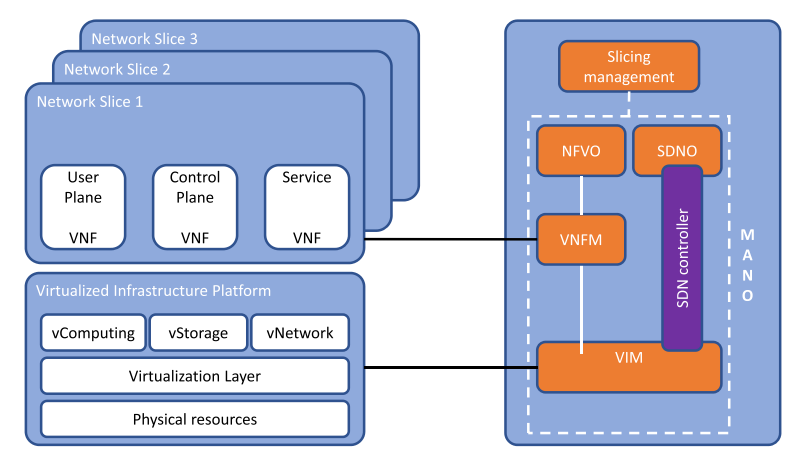
\includegraphics[width=0.9\linewidth]{../immagini/arch1}
	\caption[Architettura NS a singolo controller]{Struttura di un'architettura basata su Network Slicing a singolo proprietario e singolo controller}
	\label{fig:arch1}
\end{figure}
\begin{figure}
	\centering
	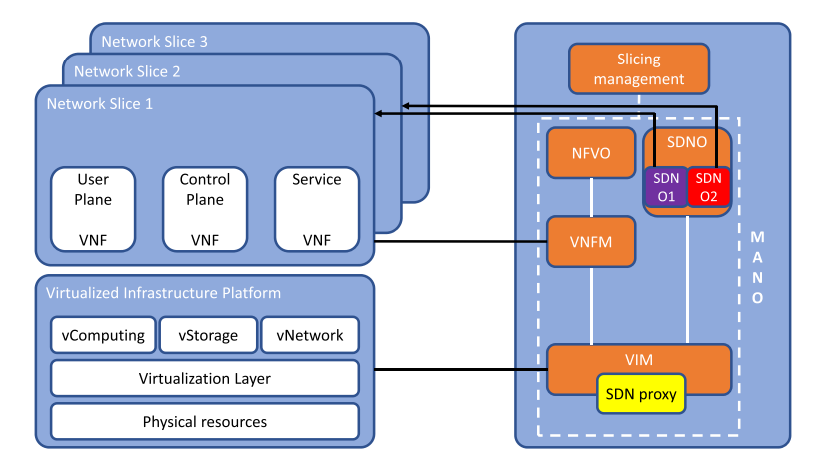
\includegraphics[width=0.9\linewidth]{../immagini/arch2}
	\caption[Architettura NS a doppio controller]{Struttura di un'architettura basata su Network Slicing a singolo proprietario e doppio controller}
	\label{fig:arch1}
\end{figure}

\section{Utilizzi e vantaggi}\label{ch:1.3}
L'idea del Network Slicing nasce con una strettissima correlazione con il 5G. Si prevede, infatti, che le reti di quinta generazione saranno in grado di creare grandi opportunità per nuove aziende e servizi. Questo porterà ad una grandissima varietà di richieste nei confronti della rete, che dovrà essere in grado di soddisfare necessità molto diverse tra loro.\\
Il Network Slicing si pone come una soluzione ideale a questo problema. La sua grande versatilità, infatti, risulta lo strumento perfetto per accontentare un'ampia gamma di richieste di varia natura. \cite{NS5g}\\\\
Queste tecnologie sono destinate ad innovare molte tipologie di comunicazione. Si prevede che un grosso impatto sarà percepito dall'industria e dai mercati verticali. Una rete flessibile e prestante ha infatti un'influenza significativa sulla produzione e permette di ottimizzare l'efficienza su tutti i livelli della filiera.\\
Un operatore può fornire al singolo cliente la gestione della propria Network Slice, permettendo di \textit{orchestrarla} a seconda delle proprie necessità. Un cliente può essere rappresentato da un'azienda che voglia basare la sua rete interna su un'infrastruttura di questo genere.\\\\
Tra i molteplici mercati che trarrebbero vantaggio da queste tecnologie possiamo evidenziare i seguenti.
\begin{itemize}
	\item \textbf{Automotive}\\
	La potenzialità più interessante delle telecomunicazioni nel campo dell'automotive è senza dubbio la comunicazione \textit{vehicle-to-everything}.\\
	Con questo termine si intende la possibilità di un veicolo di comunicare con diversi interlocutori in grado di fornire informazioni utili per comfort e sicurezza:
	\begin{itemize}
		\item L'\textit{Infotainment} è al giorno d'oggi una caratteristica imprescindibile di ogni veicolo. Una efficace comunicazione tra il veicolo e i passeggeri è fondamentale per una guida più attenta e confortevole.
		\item È opportuno anche che il veicolo sia in grado di comunicare continuamente con la casa madre, per mantenere il software e i dati sempre aggiornati.
		\item Per una maggiore sicurezza è importante garantire una comunicazione \textit{vehicle-to-vehicle} a bassissima latenza, per permettere di conoscere posizione e velocità reciproche e avere a disposizione un maggior numero possibile di dati riguardanti le condizioni della strada e del traffico.
		\item Sarebbe infine possibile offrire un'ulteriore sicurezza permettendo al veicolo di comunicare con vari sensori a terra in grado di monitorare traffico, visibilità o condizioni del manto stradale.
	\end{itemize}
	L'utilizzo per questo scopo di una rete pubblica 5g ottimizzata tramite Network Slicing permetterebbe di avere una maggiore copertura, maggiori prestazioni e un costo inferiore.
	
	\item \textbf{Energia}\\
	Una delle più importanti nuove frontiere nel campo dell'energia è rappresentata dalle \textit{Smart Grids}.\\Questo termine sta ad indicare una rete di distribuzione di energia supportata da un costante flusso di informazioni, in grado di gestire in maniera intelligente la distribuzione dell'elettricità, evitando sovraccarichi e minimizzando le perdite.\\Inoltre, con la diffusione degli impianti fotovoltaici privati, la rete deve essere in grado di convogliare adeguatamente al proprio interno l'energia prodotta.\\
	Un'infrastruttura che permetta queste operazioni al momento non esiste. Una rete 5g supportata dal Network Slicing sarebbe in grado di svolgere efficacemente queste funzioni, garantendo le prestazioni richieste.\\
	Le necessità di una rete in questo ambito sono una zona di copertura molto estesa, una bassa latenza e una grande affidabilità, anche in situazioni di emergenza.
	\begin{figure}
		\centering
		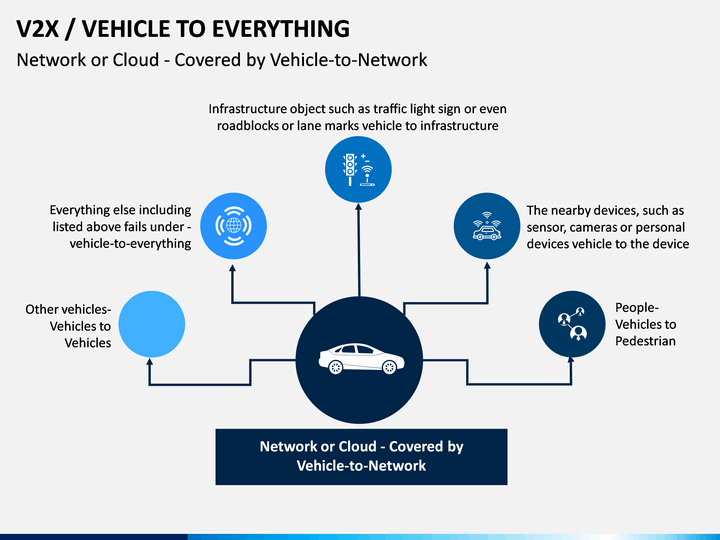
\includegraphics[width=0.75\linewidth]{../immagini/vehicle-to-everything-slide12}
		\caption[Vehicle-to-everything]{Comunicazioni di tipo Vehicle-to-Everything (V2X)}
		\label{fig:vehicle-to-everything-slide12}
	\end{figure}
	\begin{figure}
		\centering
		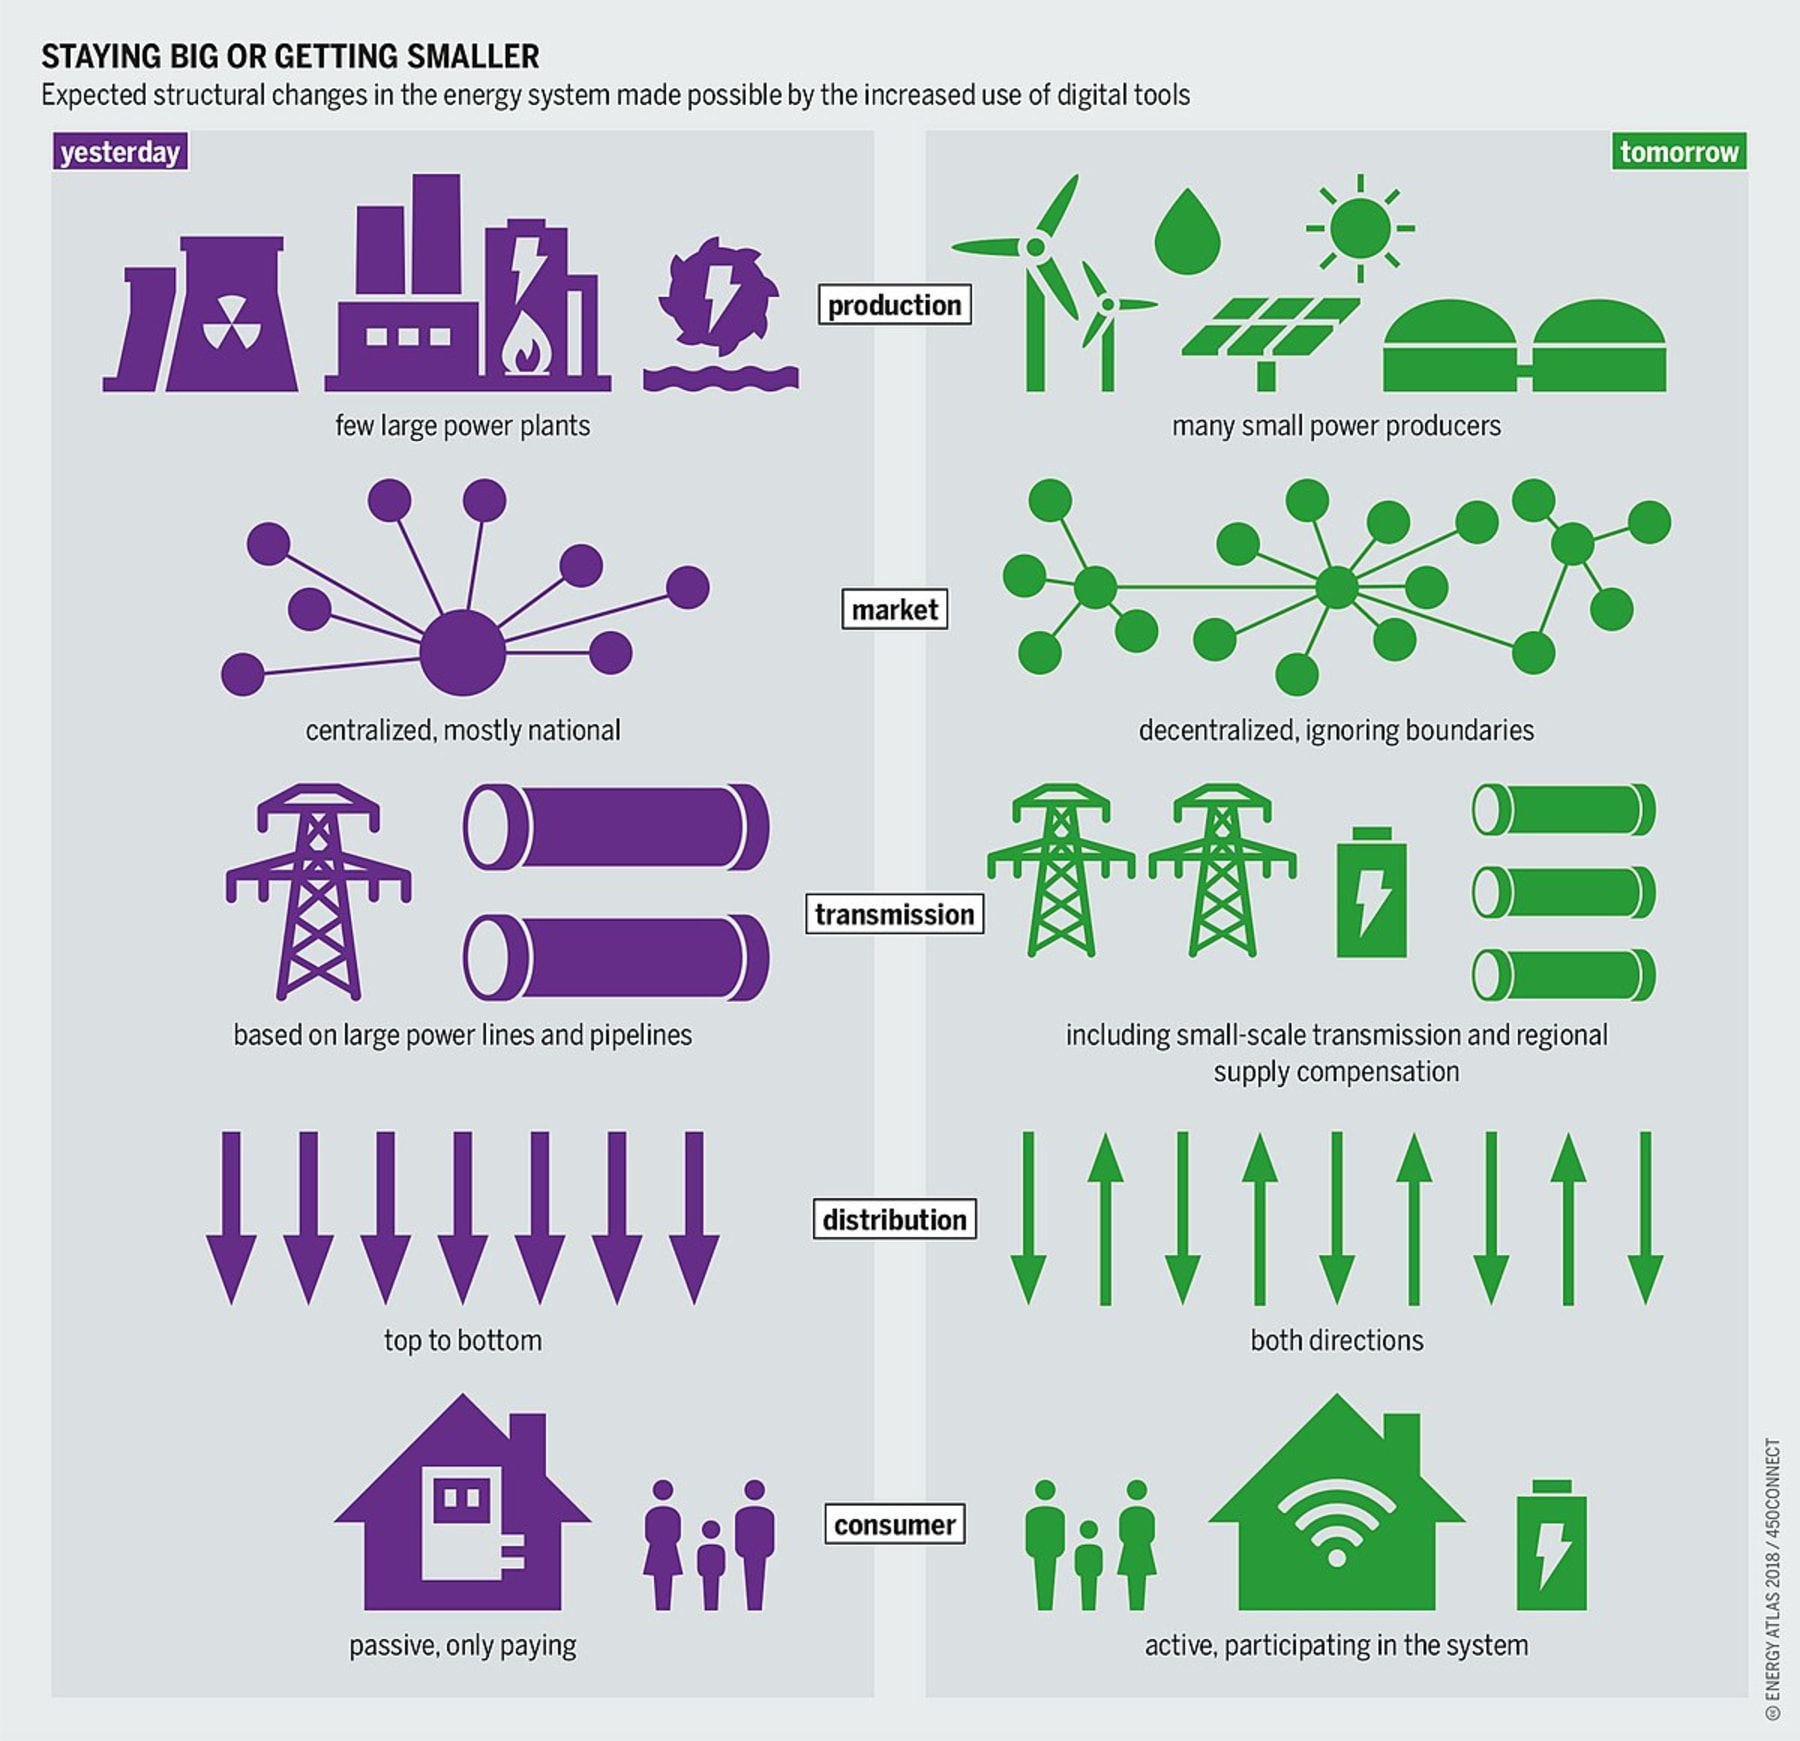
\includegraphics[width=0.75\linewidth]{../immagini/0_7i2ht2hZquYBwybh}
		\caption[Smart Grids]{Produzione e gestione dell'energia tramite Smart Grid, supportata da una rete di informazione}
		\label{fig:07i2ht2hzquybwybh}
	\end{figure}\\
	
	\item \textbf{Sanità}\\
	In ambito sanitario, l'implementazione di reti flessibili e prestanti aprirebbe tantissime opportunità.\\
	Una tra le novità sarebbe sicuramente la possibilità di monitorare in tempo reale le strumentazioni e i pazienti dentro e fuori gli ospedali.\\
	Tuttavia, risulta ancora più interessante l'idea della \textit{chirurgia da remoto}. Avere a disposizione una rete in grado di fornire una bassissima latenza, infatti, permetterebbe ai chirurghi di operare pazienti senza essere fisicamente in ospedale. Questo risulterebbe fondamentale in caso di operazioni specialistiche eseguite da esperti, riducendo drasticamente i costi per i pazienti ed eventualmente salvandone la vita.
	
	\item \textbf{IoT e Smart Cities}\\
	IoT e Smart Cities sono campi in continua espansione, per i quali una connessione su aree di grandi dimensioni risulta fondamentale. L'idea di base è di avere una vasta rete di sensori che permettano di raccogliere dati e gestire di conseguenza svariati parametri, come illuminazione o riscaldamento, in modo da avere un funzionamento ottimale e minimizzare i consumi.\\A differenza delle applicazioni precedentemente citate, la latenza non è un requisito stringente. È tuttavia fondamentale che i vari elementi della rete abbiano un basso dispendio energetico e che la copertura sia sufficiente a garantire che tutti i sensori possano comunicare.  \cite{5g5}\\
	
\end{itemize}I vantaggi apportati dal Network Slicing sono quindi numerosi e di diversa natura, a seconda del servizio richiesto e della necessità del consumatore.\\\\
Nel capitolo 3 verranno confrontate le prestazioni di una rete classica con quelle di una rete costruita seguendo i principi del Network Slicing.
	\chapter{Strumenti utilizzati}\label{ch:capitolo2}
\section{Realtà virtuale}
Il concetto di realtà virtuale non è recente come si possa pensare, le prime testimonianze risalgono al 1960 con la \textit{Telesphere Mask}, brevettata da Heiling, che era stata pensata come un apparato da collegare alla tv per simulare la sensazione di realtà muovendosi nelle tre dimensioni. Allora però non ebbe il successo sperato, il boom di questa tecnologia è arrivato solo nel 2012 con l'uscita dell'\textit{Oculus Rift} che la ha resa accessibile a milioni di utenti in tutto il mondo.\\\\
Una definizione ufficiale di realtà virtuale non esiste ancora, le più accreditate sono però quella data da Isdale nel 1998 "È la simulazione di un ambiente reale o immaginario che può essere sperimentato visivamente nelle tre dimensioni e che fornisce inoltre un'esperienza interattiva con il suono e possibilmente anche con feedback tattili o di altre forme. La realtà virtuale è un modo per gli esseri umani di visualizzare, manipolare e interagire con computer e dati estremamente complessi" e quella data da Baieier nel 1993 "È un ambiente artificiale creato con hardware e software di computer e presentato a un utente in modo tale che appaia e si senta come un ambiente reale", pertanto la realtà virtuale si riferisce a un mondo 3D completamente immersivo e interattivo creato con l'utilizzo di un calcolatore che permette all'utente, grazie all'uso di un Head Mounted Display, di entrarvi e di diventare parte attiva di esso \cite{inbook}.\\\\
L'architettura necessaria per far funzionare il tutto si compone di un visore con un campo visivo dai 100 ai 110 gradi e un frame rate compreso tra 60fps e 120fps dotato anche di sensori che permettono, insieme ad almeno due \textit{base station}, l'\textit{Head Tracking} ovvero lo spostamento dell'immagine in base alla posizione della testa. Per poter interagire effettivamente con il mondo circostante vengono utilizzati due controller, uno per mano, sempre rilevati dalle \textit{base station}.\\\\
Spesso il concetto realtà virtuale viene confuso con quello di realtà aumentata; quest'ultima però è un potenziamento della percezione del mondo reale al quale vengono aggiunti dei contenuti digitali e che non necessita di hardware appositi per funzionare ma può essere applicata anche con l'utilizzo di smartphone o tablet. Un classico esempio di realtà aumentata è un famoso gioco Nintendo uscito nel 2016, \textit{Pokemon Go}, nel quale i personaggi venivano proiettati nel mondo reale e il giocatore poteva interagire con loro e catturarli. \\\\
Anche se attualmente l'applicazione principale di questa tecnologia è nel campo videoludico ultimamente sta trovando spazio anche in altri campi come ad esempio quello dell'addestramento militare. \textit{DoDAAM}, un azienda coreana, ha già creato tutta una serie di simulazioni di situazioni di guerra come ad esempio il lancio da un aeroplano, la guida di un carro armato e di un jet riducendo contemporaneamente costi, tempi e rischi. Altre applicazioni si possono trovare nel ambito medico sopratutto nella terapia di disturbi psichiatrici e nella riabilitazione motoria e cognitiva. Le potenzialità della realtà virtuale possono essere usate anche nella formazione del personale medico simulando, ad esempio, un operazione chirurgica.	
\subsection{Htc Vive Pro}
\begin{figure}[h!]
	\centering
	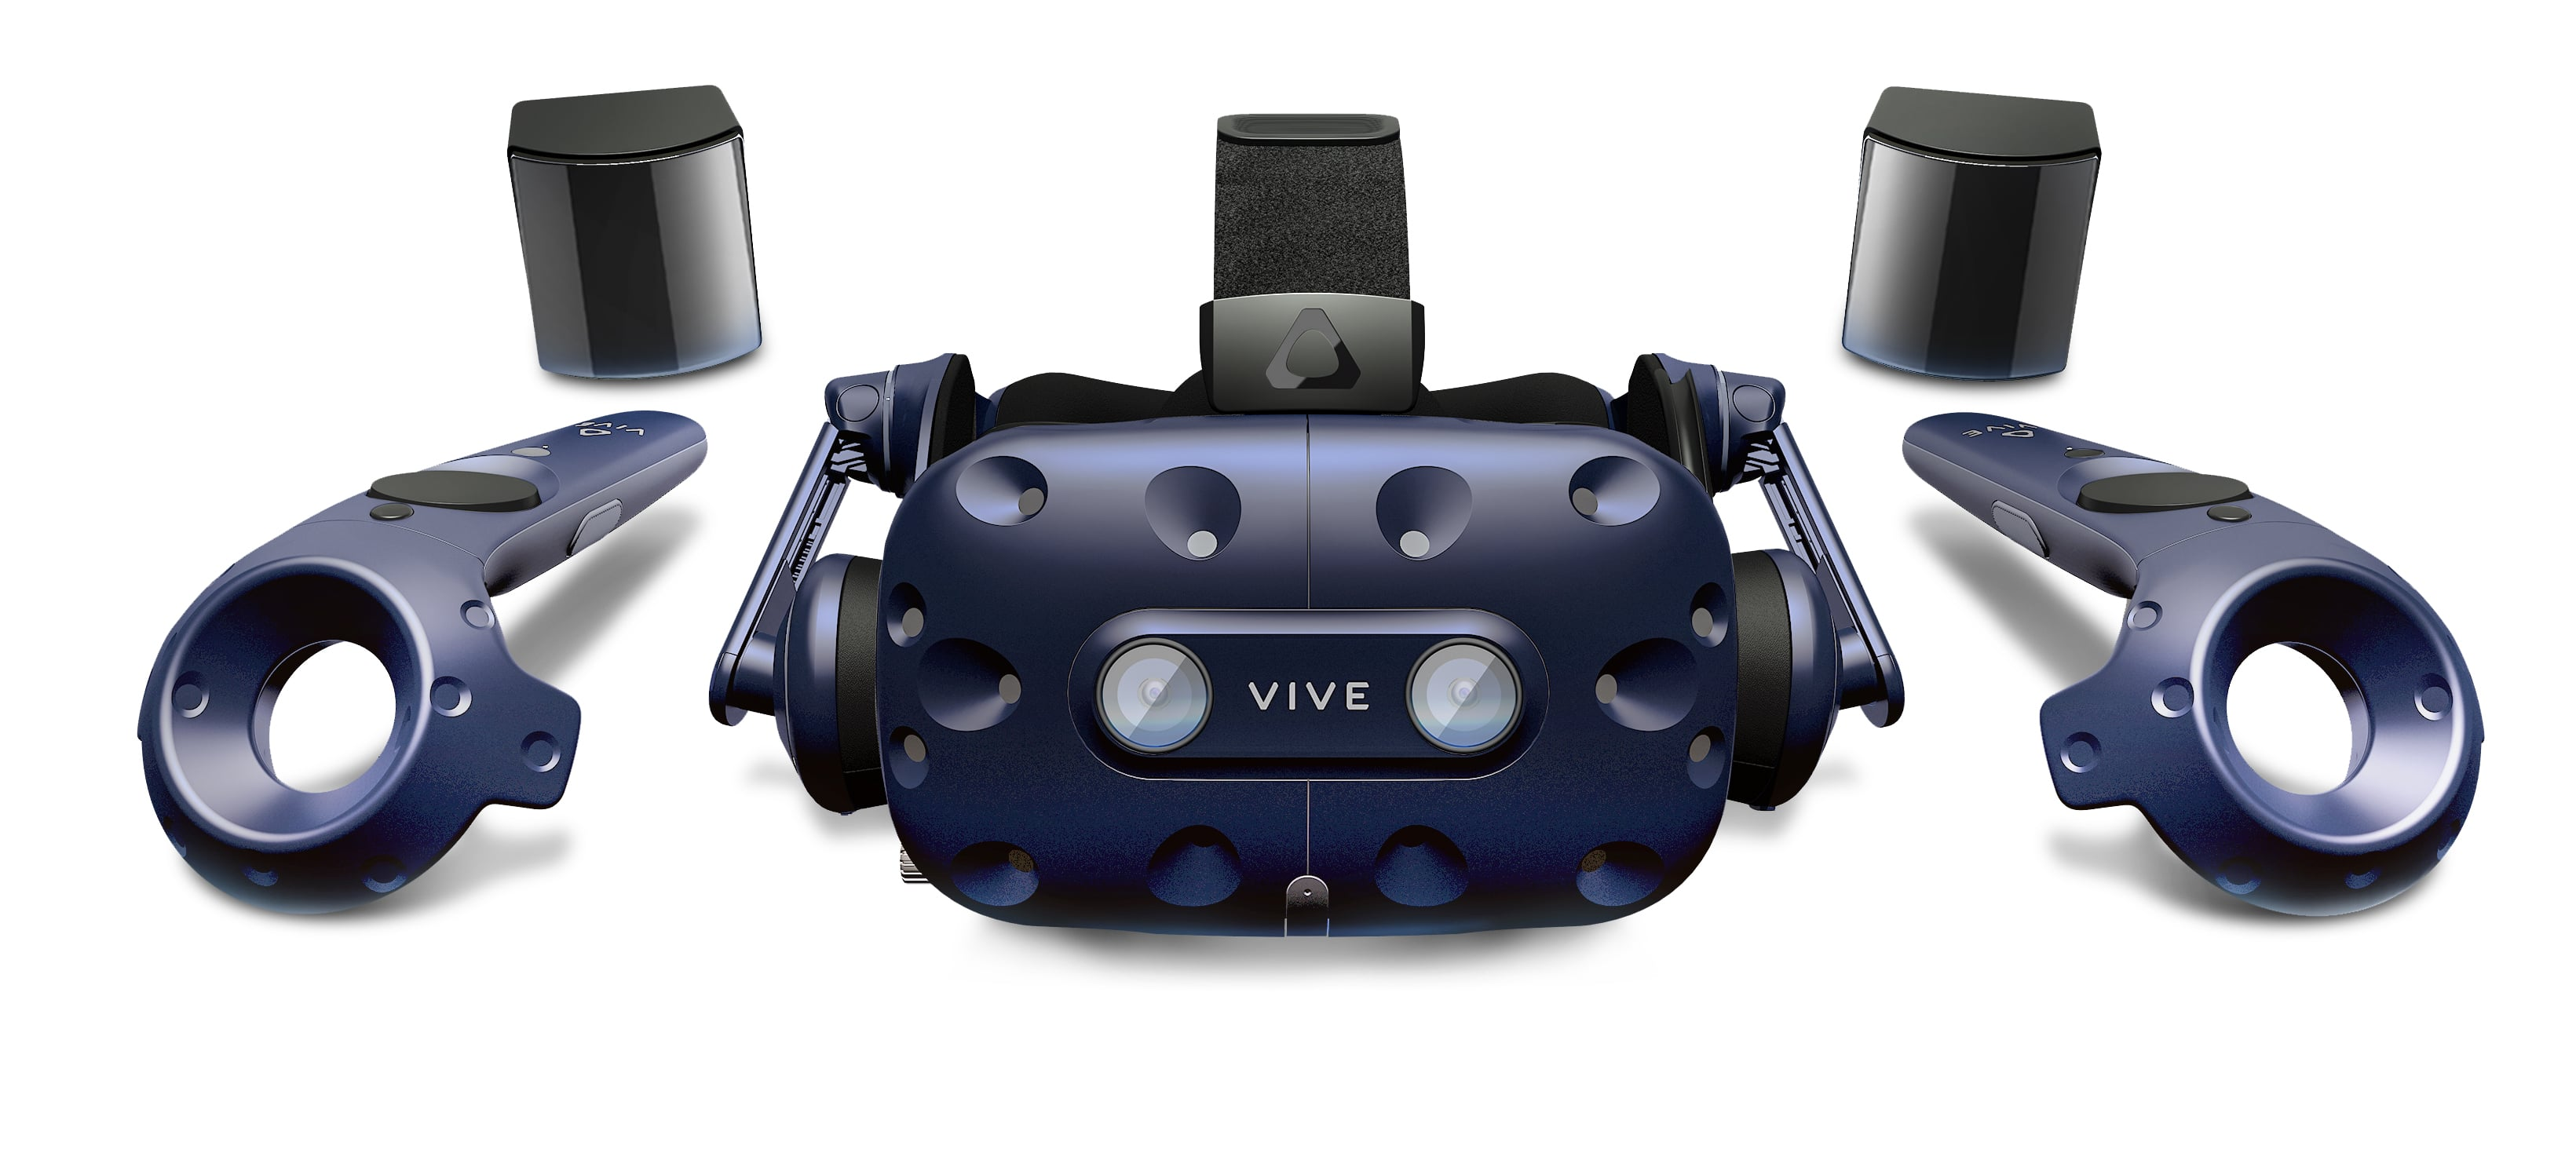
\includegraphics[width=1\linewidth]{../immagini/vive}
	\caption[Htc Vive]{Visore e componenti }
	\label{fig:vive}
\end{figure}
Il sistema di realtà virtuale utilizzato durante la realizzazione del progetto è l'HTC Vive Pro, prodotto da HTC e Valve, (in Figura 2.1) e commercializzato a partire dal 2016. Il visore VIVE presenta due lenti Fresnel non perfettamente circolari ma con un lato piatto che le allinea con il naso permettendo anche di avvicinarle o allontanarle tra loro permettendo di adattarle alla propria distanza interpupillare. L'HMD presenta oltre ai 32 sensori infrarossi per il tracking posizionati sulla superficie anche un giroscopio, un accelerometro e un sensore di posizione laser per riprodurre nella maniera più fedele possibile il movimento della testa.\\
I \textit{controller} servono per interagire con l'ambiente e sono dotati di 24 sensori per il tracking oltre che a una serie di tasti.\\
Le \textit{Base Station} sono degli emettitori, generano una luce ad infrarossi e due fasci laser che vengono rilevati dai sensori posti su controller e HMD. Basandosi poi sulla posizione di questi sensori e su quanto sono stati irradiati è possibile stimare con un ottima precisione la posizione e l'orientamento degli oggetti rispetto alle base station.\\\\
Per la configurazione di questo strumento ci si avvale di un runtime chiamato \textit{SteamVR} ncluso nel client di Steam che consente di usufruire della realtà virtuale. SteamVR viene installato automaticamente quando Steam rileva la connessione di un visore al PC dell'utente, ma può essere installato anche manualmente.\\
SteamVR consente all'utente la gestione di molti aspetti della sua esperienza di gioco tra cui:
\begin{itemize}
	\item Configurazione della stanza, con cui definire la propria area di gioco.
	\item Controllo stato e gestione del dispositivo, con cui aggiornare il firmware, associare nuovi dispositivi, cambiare le impostazioni audio, impostare la duplicazione e personalizzare funzionalità quali il Motion Smoothing \cite{steamvr}.
\end{itemize}
Attualmente è uno dei migliori dispositivi disponibili sul mercato e come tale per funzionare il pc su cui far girare il tutto deve soddisfare alcuni requisiti. Di seguito vengono riportati quelli consigliati presi direttamente dal sito ufficiale della Vive:
\begin{itemize}
	\item \textbf{Processore} Intel Core i5 o superiore
	\item \textbf{GPU} NVIDIA GeForce GTX 1070/Quadro P5000, AMD Radeon Vega 56 o superiore
	\item \textbf{Memoria} 4Gb di RAM o più
	\item \textbf{Video Output} DisplayPort 1.2 o più recente
	\item \textbf{USB port} 1x USB 3.0 o più recente
	\item \textbf{O.S.} Windows 10
\end{itemize} 

\section{Unity 3D}
Unity è un motore grafico sviluppato da Unity Technologies usato principalmente per sviluppare videogiochi e simulazioni in grafica 2D o 3D tramite scripting in C\#. È un ambiente multi-piattaforma che permette la creazione di applicazioni per diversi dispositivi tra cui: Android, iOS, Windows, Playstation e sviluppo di software di realtà virtuale e aumentata. Unity nel suo Asset Store mette a disposizione tutta una serie di librerie, modelli, prefab e script sia gratuiti che a pagamento. Tra questi nel progetto viene utilizzato OpenVR ovvero un API che consente alle applicazioni di interagire con gli hardware di diversi produttori senza necessità di rilevare l'effettivo hardware puntato. Supporta diversi HMD tra cui Valve Index, HTC Vive, Oculus Rift, Windows Mixed Reality e altri.
\section{Blender}
Blender è una suite di creazione 3D gratuita e open source. Il software mette a disposizione diverse funzionalità tra cui modellazione 3D, texuring, simulazione di elementi come corpi rigidi, fluidi e fumi, animazione 3D, rendering ecc.\\
Nel progetto servirà per la gestione di tutti i dati 3D in particolare per la fase di pre-process per creare la scena e nella fase di post-process per visualizzare e maneggiare i risultati. 
\subsection{Modelli 3D} 
\begin{figure}
	\centering
	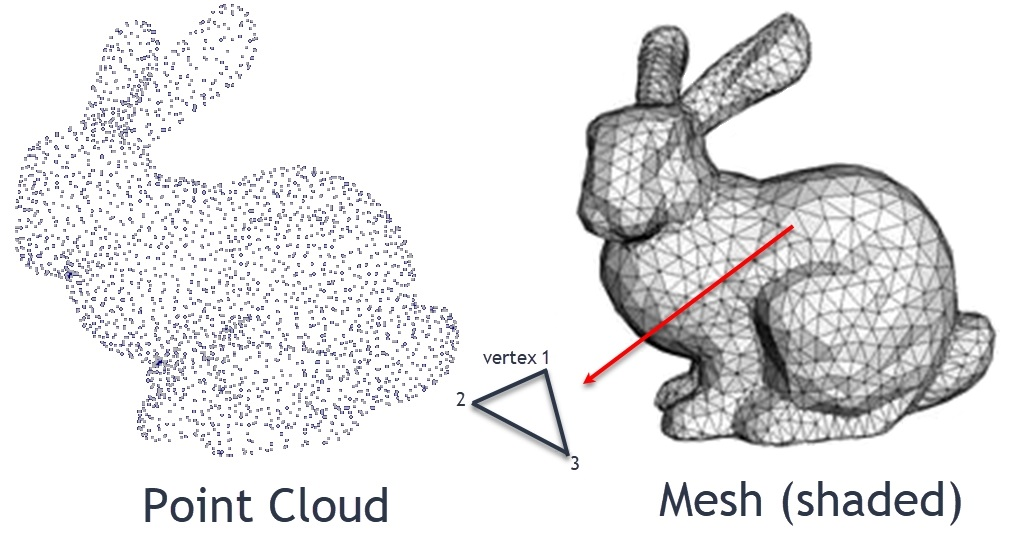
\includegraphics[width=0.8\linewidth]{../immagini/meshpoint}
	\caption[Mesh e Pointcloud]{Esempio di mesh e pointcloud }
	\label{fig:meshpoint}
\end{figure}
Tra i vari modelli 3D che si possono trovare nella computer grafica e che durante la realizzazione del progetto sono stati particolarmente ricorrenti troviamo \textit{mesh} e \textit{poitncloud}.\\
Una mesh poligonale, detta anche maglia poligonale, è una collezione di vertici, spigoli e facce che definiscono la forma di un oggetto poliedrico. . Le facce consistono, di
solito, di rettangoli, triangoli, o altri semplici
poligoni convessi, dal momento che ci`o
semplifica il rendering.\\
Una mesh poligonale si compone di tre tipi di elementi:
\begin{itemize}
	\item Il \textbf{vertice} è una posizione nello spazio e ha
	informazioni relative al colore e al vettore normale.
	\item Il \textbf{lato} è il collegamento tra due vertici.
	\item La \textbf{faccia} un insieme chiuso di lati, ad esempio una faccia triangolare avrà tre lati e una faccia quadrangolare avrà quattro lati. Un poligono è un insieme complanare di facce. Ogni faccia ha inoltre anche un vettore normale alla sua superficie. 
\end{itemize}
Una point cloud, invece, è un insieme di punti nello spazio non dotato di informazioni topologiche (niente lati ne triangoli), questo tipo di dati proviene dall'utilizzo di scanner 3D o sensori come il Kinect.  	 


	\chapter{Esempio pratico}\label{ch:capitolo3}

\section{Idea di base}\label{ch:3.1}
Nei precedenti capitoli abbiamo evidenziato come al giorno d'oggi una rete debba essere sempre più flessibile ed in grado di fornire le prestazioni più adeguate ad un servizio richiesto.\\
Abbiamo poi visto alcuni strumenti di simulazione che ci permettono di analizzare il funzionamento di reti di varia natura, in particolare le reti di tipo SDN per le quali i programmi citati sono ideali. Abbiamo infine esaminato diversi metodi per poter misurare le prestazioni della nostra rete, con un particolare interesse nei confronti degli strumenti che ci permettono di valutare il comportamento della rete rispetto ad uno specifico servizio.\\\\
Avendo a disposizione conoscenze e competenze nell'ambito delle reti SDN e del Network Slicing, è ora interessante simulare e confrontare due diverse reti, di uguale topologia, delle quali solo ad una verranno applicati i principi del Network Slicing.
\section{Realizzazione}\label{ch:3.2}
La topologia in esame ha una struttura piuttosto semplice: sono presenti due host, i quali dovranno comunicare tramite diverse porte TCP, ciascuna associata ad un servizio.\\\\
Queste porte sono state scelte come esempi di applicazioni che richiedono prestazioni diverse:\\
\begin{itemize}
	\item \textbf{Porta 20: FTP}\\
	FTP (File Transfer Protocol), è un protocollo di trasferimento dati. Possiamo considerare FTP come un esempio di servizio che richiede una banda importante, per permettere un veloce trasferimento dei dati e dei file.\\
	\item \textbf{Porta 5000: Chat, streaming e gaming}\\
	La porta 5000 è utilizzata da varie applicazioni di diverse tipologie, come chat, videochat, streaming video e gaming. Tutti questi servizi sono accomunati dalla necessità di avere una comunicazione a bassa latenza.\\
\end{itemize}
Ovviamente esiste un enorme numero di possibili servizi. Per semplicità e chiarezza verranno usati solo questi tre, ma il processo è facilmente scalabile.\\
\subsection{Topologia}\label{ch:3.2.1}
Il Network Slicing prevede che una rete sia in grado di allocare le risorse necessarie affinché una specifica applicazione abbia a disposizione una rete ottimizzata per le sue necessità.\\
Ai fini di una dimostrazione efficace è quindi opportuno creare una topologia che sia in grado di fornire sia una bassa latenza sia una larga banda.\\\\
La topologia che andremo ad esaminare è composta da due host, collegati da quattro switch. Tra host e switch sono presenti collegamenti con diverse caratteristiche. Questa semplice rete verrà poi programmata affinchè le prestazioni che la rete è in grado di fornire siano ripartite al meglio tra i vari servizi.\\\begin{figure}[H]
	\centering
	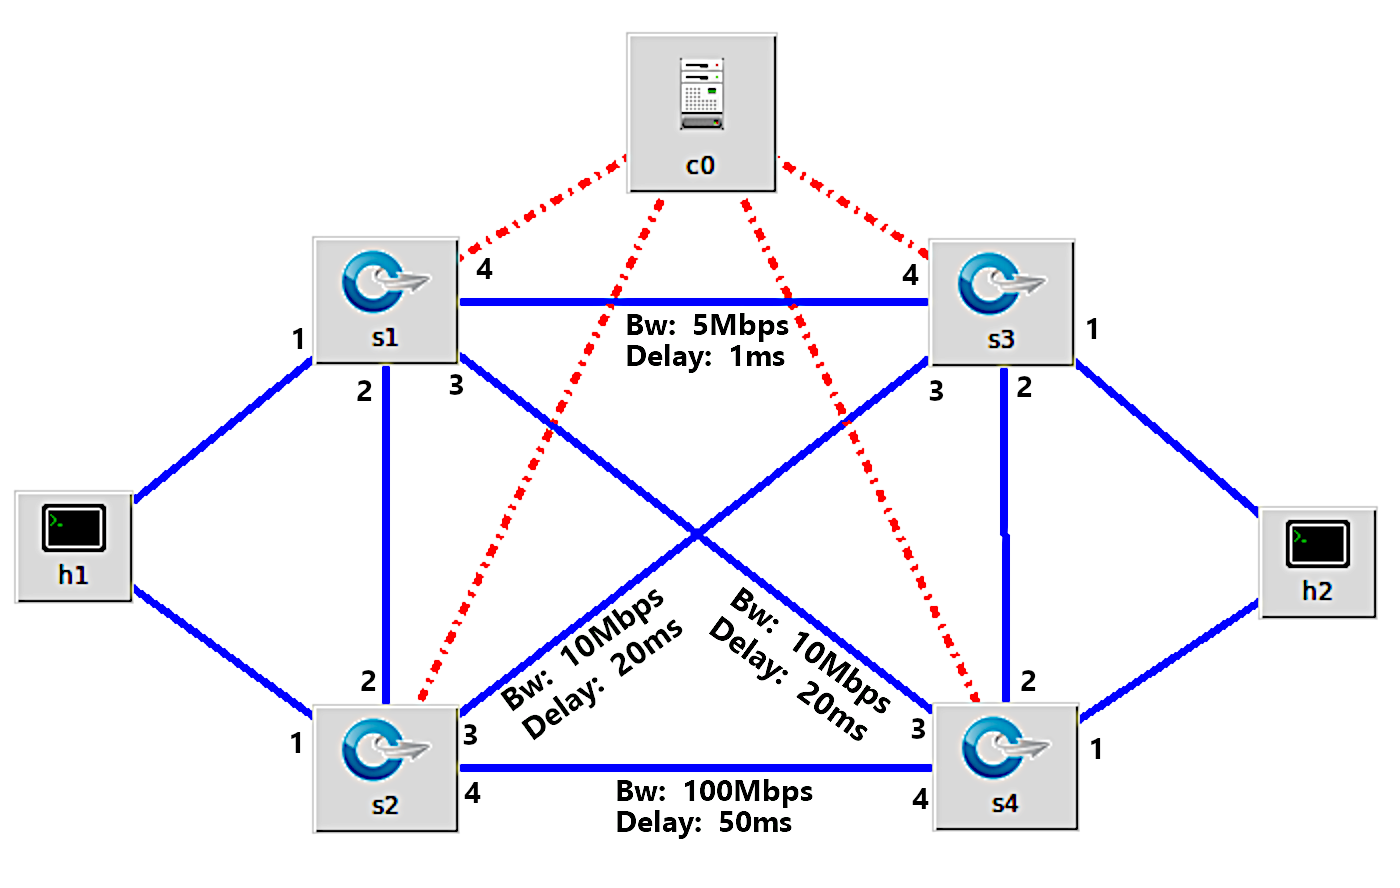
\includegraphics[width=1\linewidth]{../immagini/esempio/topo}
	\caption[Topologia d'esempio]{Topologia della rete in esame}
	\label{fig:topo}
\end{figure}
Come illustrato nel capitolo precedente, per costruire la topologia è necessario avvalersi di uno Script Python.\\Questo script verrà salvato nel file \textit{test.py}\\

\begin{lstlisting}[language=Python,numbers=left,firstnumber=1,stepnumber=1]
from mininet.topo import Topo
from mininet.link import TCLink
	
class MyTopo( Topo ):
	"Simple topology example."
	
	def __init__( self ):
		"Create custom topo."
	
		# Initialize topology
		Topo.__init__( self )
	
		# Add hosts and switches
		h1 = self.addHost( 'h1' )
		h2 = self.addHost( 'h2' )
		s1 = self.addSwitch( 's1' )
		s2 = self.addSwitch( 's2' )
		s3 = self.addSwitch( 's3' )
		s4 = self.addSwitch( 's4' )
	
		# Add links
		self.addLink( h1, s1, 1, 1, bw=100, delay='1ms' )
		self.addLink( h1, s2, 2, 1, bw=100, delay='1ms' )
		self.addLink( h2, s3, 1, 1, bw=100, delay='1ms' )
		self.addLink( h2, s4, 2, 1, bw=100, delay='1ms' )
		self.addLink( s1, s2, 2, 2, bw=100, delay='1ms' )
		self.addLink( s3, s4, 2, 2, bw=100, delay='1ms' )
		
		self.addLink( s1, s3, 4, 4, bw=5, delay='1ms' )
		self.addLink( s1, s4, 3, 3, bw=10, delay='20ms' )
		self.addLink( s2, s3, 3, 3, bw=10, delay='20ms' )
		self.addLink( s2, s4, 4, 4, bw=100, delay='50ms' )
	
topos = { 'mytopo': ( lambda: MyTopo() ) }
\end{lstlisting}
Possiamo notare alcune differenze con il codice di esempio fornito nel capitolo precedente.\\
Nella creazione dei link, infatti, viene specificate le porte di ciascun nodo a cui ciascun ramo è collegato.\\
Per le connessioni create nelle righe 29, 30, 31 e 32, inoltre, sono state specificate banda e latenza, coerentemente con i dati della figura 3.1, mentre per le altre sono stati scelti come parametri standard 100Mbps di banda e 1ms di latenza.\\
A causa di questa differenza, è necessario importare ulteriori API, operazione che viene svolta alla riga 2.\\\\
Ai fini della dimostrazione è necessario creare due reti distinte, una classica e una di tipo SDN. Lo script Python deve quindi essere eseguito in due modi diversi.
\begin{itemize}
	\item Per creare una topologia classica si usa il comando
	\begin{center}
		\textbf{sudo mn --custom test.py --topo mytopo --link tc}
	\end{center}
	che avvia Mininet con la topologia \textit{"mytopo"} del file \textit{"test.py"}\\
	Da notare il parametro \textit{--link} che deve essere posto \textit{"tc"} per permettere la personalizzazione di banda e latenza.\\
	\item Per creare una topologia SDN bisogna invece scrivere
	\begin{center}
		\textbf{sudo mn --custom test.py --topo mytopo --link tc --switch ovsk}
	\end{center}
	specificando quindi che gli switch debbano supportare OpenFlow.\\
\end{itemize}

\subsection{Forwarding}\label{ch:3.2.2}
È ora necessario configurare gli switch affinché la rete possa essere ottimizzata per i servizi richiesti.\\
Perchè avvenga è necessario che i pacchetti che richiedono una bassa latenza, rappresentati dai servizi sulla porta TCP 5000, siano inviati sul ramo che collega s1 a s3, mentre per i servizi che necessitano di molta banda, rappresentati dai pacchetti \textit{FTP}, è necessario che le informazioni viaggino sul ramo che collega s2 e s4.\\
I rami che collegano s1 con s2 e s3 con s4 sono dedicati a spostare i pacchetti verso il migliore tra i due percorsi.\\\\
Per configurare gli switch utilizziamo i comandi presentati nel capitolo precedente, con sintassi di questo tipo:\\
\begin{center}
	\textbf{ovs-ofctl add-flow [switch] priority=[priorità],in\_port=[porta switch],tcp,tcp\_src=[porta TCP],actions=output:[porta switch] }\\
\end{center}
Analizziamo il parametri del comando:\\
\begin{itemize}
	\item \textit{priority} definisce la priorità dell'azione. Un comando con priorità alta prevale su uno con priorità bassa.\\
	\item \textit{in\_port} specifica in quale porta dello switch debbano entrare i pacchetti appartenenti al flusso\\
	\item \textit{tcp\_src} specifica quale porta TCP stiano usando i pacchetti appartenenti al flusso\\
	\item \textit{output} definisce su quale porta dello switch dovranno essere reindirizzati i pacchetti in uscita\\
\end{itemize}
Per comodità, tutti i comandi necessari vengono racchiusi in uno script chiamato \textit{test.sh}, che presenta il seguente contenuto
\begin{lstlisting}[language=bash,numbers=left,firstnumber=1,stepnumber=1]
#Elimino i flussi preesistenti
sudo ovs-ofctl del-flows s1
sudo ovs-ofctl del-flows s2
sudo ovs-ofctl del-flows s3
sudo ovs-ofctl del-flows s4

#Creo un collegamento tra gli switch e i propri host
sudo ovs-ofctl add-flow s1 priority=1,actions=output:1
sudo ovs-ofctl add-flow s2 priority=1,actions=output:1
sudo ovs-ofctl add-flow s3 priority=1,actions=output:1
sudo ovs-ofctl add-flow s4 priority=1,actions=output:1

#Creo un canale di default
sudo ovs-ofctl add-flow s1 priority=2,in_port=1,actions=output:3
sudo ovs-ofctl add-flow s2 priority=2,in_port=1,actions=output:3
sudo ovs-ofctl add-flow s3 priority=2,in_port=1,actions=output:3
sudo ovs-ofctl add-flow s4 priority=2,in_port=1,actions=output:3

#Sposto i pacchetti verso le linee ottimizzate
sudo ovs-ofctl add-flow s1 
	priority=4,dl_type=0x0800,nw_proto=6,in_port=1,tcp,tcp_dst=20,
	actions=output:2
sudo ovs-ofctl add-flow s3 
	priority=4,dl_type=0x0800,nw_proto=6,in_port=1,tcp,tcp_dst=20,
	actions=output:2
sudo ovs-ofctl add-flow s2 
	priority=4,dl_type=0x0800,nw_proto=6,in_port=1,tcp,tcp_dst=5000,
	actions=output:2
sudo ovs-ofctl add-flow s4 	
	priority=4,dl_type=0x0800,nw_proto=6,in_port=1,tcp,tcp_dst=5000,
	actions=output:2

#Trasferisco i pacchetti sulle linee ottimizzate
sudo ovs-ofctl add-flow s1 
	priority=3,dl_type=0x0800,nw_proto=6,in_port=1,tcp,tcp_dst=5000,
	actions=output:4
sudo ovs-ofctl add-flow s3 
	priority=3,dl_type=0x0800,nw_proto=6,in_port=2,tcp,tcp_dst=5000,
	actions=output:4
sudo ovs-ofctl add-flow s2 
	priority=3,dl_type=0x0800,nw_proto=6,in_port=2,tcp,tcp_dst=20,
	actions=output:4
sudo ovs-ofctl add-flow s4 
	priority=3,dl_type=0x0800,nw_proto=6,in_port=1,tcp,tcp_dst=20,
	actions=output:4

sudo ovs-ofctl dump-flows s1
sudo ovs-ofctl dump-flows s2
sudo ovs-ofctl dump-flows s3
sudo ovs-ofctl dump-flows s4
\end{lstlisting}
Per avviare lo script è necessario renderlo eseguibile. Per farlo bisogna scrivere nella CLI
\begin{center}
	\textbf{sudo chmod +X \textit{test.sh}}
\end{center}
Il comando per avviare lo script invece è
\begin{center}
	\textbf{sudo bash ./\textit{test.sh}}
\end{center}
Le righe tra 2 e 5 servono per eliminare eventuali flussi preesistenti.\\
Le righe tra 8 e 17 creano un collegamento di default, per permettere ai servizi sconosciuti di poter giungere a destinazione.\\
I comandi nelle righe tra 20 e 31 servono per permettere ai pacchetti di giungere sulla linea più adatta al servizio richiesto.\\
Le righe tra 34 e 45 compiono il vero e proprio trasferimento delle informazioni sulla linea. Una volta giunte allo switch successivo, queste vengono portate all'host grazie ai flussi precedentemente creati.\\\\
Per analizzare come le prestazioni vengano modificate dalla programmazione della rete misuriamo latenza e banda della rete per i diversi servizi prima e dopo l'esecuzione dello script.\\
Per un corretto inoltro delle informazione attraverso gli switch anche senza una programmazione tramite controller è necessario attivare l'\textit{STP (Spanning Tree Protocol)}, che permette alla rete di stabilire un percorso per collegare i due host, interrompendo gli altri collegamenti.\\
Se si prova ad usare il comando \textit{pingall} subito dopo aver costruito la topologia, infatti, possiamo notare che gli host non sono in grado di comunicare.\\
\begin{figure}[H]
	\centering
	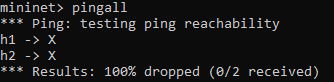
\includegraphics[width=0.9\linewidth]{../immagini/esempio/stp_off}
	\caption[Pingall con STP disattivato]{Il comando "pingall" ci permette di vedere che gli host non riescono ad inviarsi informazioni}
	\label{fig:stpoff}
\end{figure}
È quindi necessario attivare l'STP. Per farlo, bisogna usare uno specifico comando, anche in questo caso presentato in uno script per semplicità.\\
\begin{lstlisting}[language=bash]
sudo ovs-vsctl set Bridge 's1' stp_enable=true
sudo ovs-vsctl set Bridge 's2' stp_enable=true
sudo ovs-vsctl set Bridge 's3' stp_enable=true
sudo ovs-vsctl set Bridge 's4' stp_enable=true
\end{lstlisting}
Una volta attivato l'STP, la rete stabilisce un percorso tra i due host, che riescono finalmente a comunicare. Tuttavia, è importante notare che, così facendo, la maggior parte delle risorse rimangono inutilizzate.\\\\
Come sarà evidente in fase di analisi prestazionale, il collegamento tra i due host può coincidere con uno dei percorsi della rete SDN.\\
Tuttavia, gli aspetti che si vogliono evidenziare con questa dimostrazione non sono le differenze delle prestazioni in senso assoluto, ma l'incapacità di una rete classica di adattarsi allo specifico servizio richiesto.\\\\
Possiamo riutilizzare il comando \textit{pingall} per testare nuovamente il funzionamento della rete.
\begin{figure}[H]
	\centering
	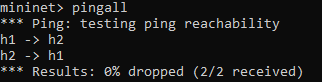
\includegraphics[width=0.9\linewidth]{../immagini/esempio/stp_on}
	\caption[Pingall con STP attivato]{Dopo aver attivato l'STP esiste un percorso tra i due host}
	\label{fig:stpon}
\end{figure}

\section{Prestazioni}\label{ch:3.3}
Avendo a disposizione la rete programmata ed un'alternativa non ottimizzata, è possibile raccogliere dei dati riguardanti le prestazioni tramite gli strumenti presentati nel capitolo precedente.
\subsection{Latenza}\label{ch:3.3.1}
\begin{figure}[H]
	\centering
	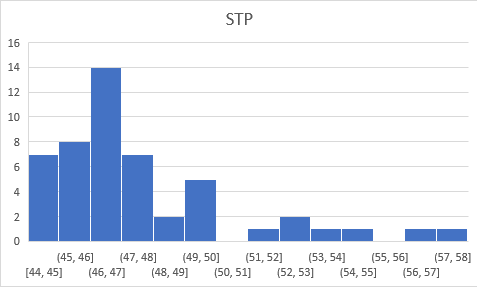
\includegraphics[width=0.9\linewidth]{../immagini/esempio/ping_stp}
	\caption[Latenza STP]{Latenza misurata su 50 misurazioni con la topologia basata su STP}
	\label{fig:pingstp}
\end{figure}
\begin{figure}[H]
	\centering
	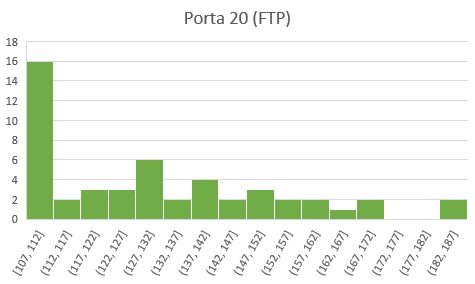
\includegraphics[width=0.9\linewidth]{../immagini/esempio/ping_ftp}
	\caption[Latenza Porta 20]{Latenza misurata su 50 misurazioni con il percorso ottimizzato per la porta 20}
	\label{fig:pingftp}
\end{figure}
\begin{figure}[H]
	\centering
	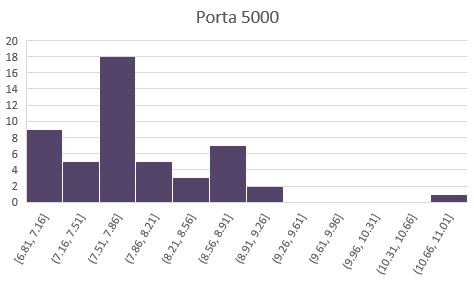
\includegraphics[width=0.9\linewidth]{../immagini/esempio/ping_5000}
	\caption[Latenza Porta 5000]{Latenza misurata su 50 misurazioni con il percorso ottimizzato per la porta 5000}
	\label{fig:ping5000}
\end{figure}
\begin{figure}[H]
	\centering
	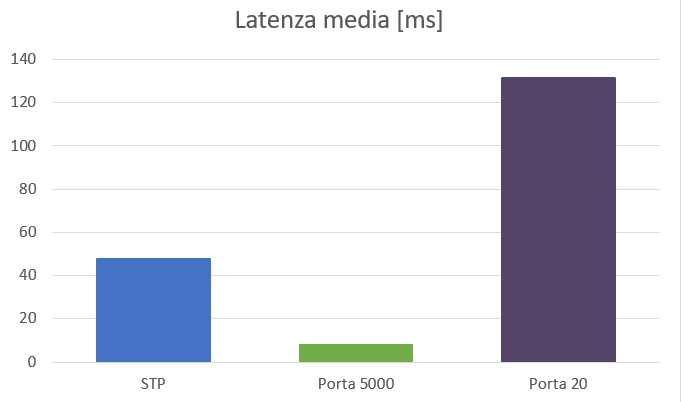
\includegraphics[width=0.9\linewidth]{../immagini/esempio/ping_medio}
	\caption[Latenza media]{Latenza media misurata su 50 misurazioni per ogni servizio}
	\label{fig:pingmedio}
\end{figure}
Possiamo osservare che il percorso stabilito tramite Spanning Tree Protocol coincide con il percorso che, nella rete programmata, viene svolto dai pacchetti di servizi non specificati.\\
\subsection{Banda}\label{ch:3.3.2}
\begin{figure}[H]
	\centering
	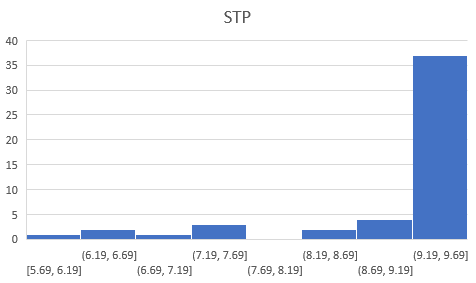
\includegraphics[width=1\linewidth]{../immagini/esempio/bw_stp}
	\caption[Banda STP]{Banda misurata su 50 misurazioni con la topologia basata su STP}
	\label{fig:bwstp}
\end{figure}
\begin{figure}[H]
	\centering
	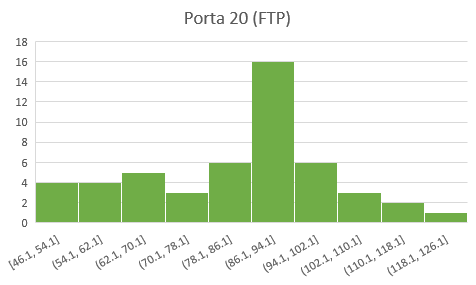
\includegraphics[width=1\linewidth]{../immagini/esempio/bw_ftp}
	\caption[Banda Porta 20]{Banda misurata su 50 misurazioni con il percorso ottimizzato per la porta 20}
	\label{fig:bwftp}
\end{figure}
\begin{figure}[H]
	\centering
	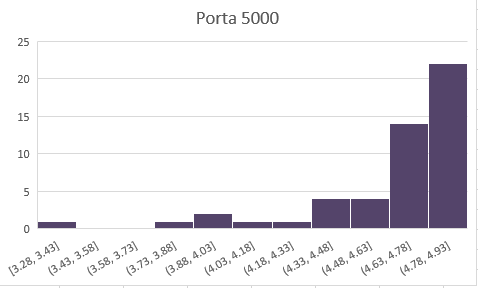
\includegraphics[width=1\linewidth]{../immagini/esempio/bw_5000}
	\caption[Banda Porta 5000]{Banda misurata su 50 misurazioni con il percorso ottimizzato per la porta 5000}
	\label{fig:bw5000}
\end{figure}
\begin{figure}[H]
	\centering
	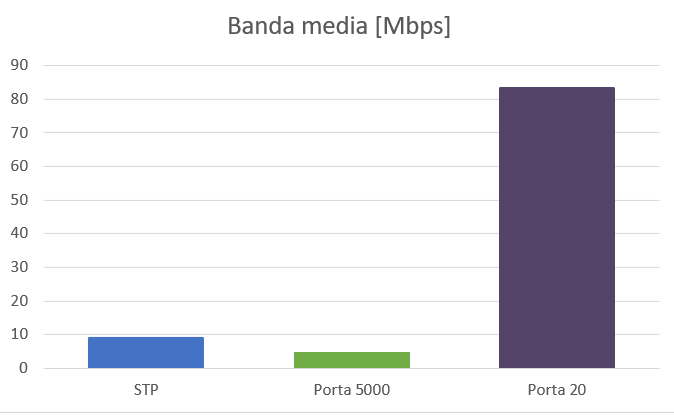
\includegraphics[width=1\linewidth]{../immagini/esempio/bw_media}
	\caption[Banda media]{Banda media misurata su 50 misurazioni per ogni servizio}
	\label{fig:bwmedia}
\end{figure}

È possibile notare come le prestazioni della rete standard non siano necessariamente peggiori rispetto alla rete programmata. È importante però osservare come queste non dipendano dallo specifico servizio richiesto e non siano quindi in grado di accontentare al meglio le diverse esigenze.
	\chapter*{Conclusione}
\addcontentsline{toc}{chapter}{Conclusione}
\phantomsection
\chaptermark{Conclusione}

In questo elaborato è stato presentato il concetto di Network Slicing e come il suo impatto potrebbe influenzare diverse tipologie di servizi.\\
È stato poi analizzato un potente strumento di simulazione, Mininet, mostrandone alcuni utilizzi di base e spiegandone le affinità con le reti di tipo SDN. Sono stati mostrati anche diversi metodi per analizzare alcune tra le prestazioni che una rete può essere in grado di offrire.\\
Questi concetti e questi strumenti sono stati poi uniti per la creazione di una rete basata sull'idea di Network Slicing, dando la possibilità di osservare come questa tipologia di architettura possa impattare la costruzione, la gestione e soprattutto l'utilizzo di un'infrastruttura.\\\\
L'esempio svolto riguarda una rete piuttosto semplice. Tuttavia, queste tecnologie possono essere usate per progettare, simulare ed infine costruire reti di dimensioni e complessità molto maggiori, andandone ad influenzare molto sensibilmente l'efficienza e le prestazioni. 
	
	\bibliographystyle{ieeetr}
	\bibliography{Bibliografia}
	
	%-----Aggiungo all'indice la voce Bibliografia ---------------------
	%%\special{pdf: out 0 << /Title (Bibliografia) /Dest [@thispage/FitH @ypos ]>>}
	\phantomsection
	\addcontentsline{toc}{chapter}{Bibliografia}
	%-------------------------------------------------------------------
	
	\newpage
	\thispagestyle{empty}
	
\end{document}
